\documentclass{article}

\usepackage{PRIMEarxiv}
\usepackage[utf8]{inputenc}
\usepackage[T1]{fontenc}
\usepackage{hyperref}
\usepackage{url}
\usepackage{amsmath}
\usepackage{booktabs}
\usepackage{amsfonts}
\usepackage{nicefrac}
\usepackage{microtype}
\usepackage{fancyhdr}
\usepackage{graphicx}
\graphicspath{{./images/}}

\pagestyle{fancy}
\thispagestyle{empty}
\rhead{ \textit{ }}
\fancyhead[LO]{Structural Recovery and Functional Reintegration in Recurrent SNNs}

\title{Structural Recovery and Functional Reintegration Dynamics under Attractor Constraints in Recurrent Spiking Neural Networks via Recurrent Potential Diffusion}

\author{
  Fumiaki INOUE \\
  \texttt{finou882@github} \\
}

\begin{document}
\maketitle

\begin{abstract}
In Spiking Neural Networks (SNNs), Winner-Take-All (WTA) competition promotes sparse representation but often drives a subset of neurons into permanent silence (the dead-neuron problem), reducing network capacity. This study proposes Targeted Recurrent Reactivation (TRR), a recurrent potential diffusion mechanism that leverages synaptic traces to diffuse membrane potentials into inactive units. We investigate the dynamics of structural recovery and functional reintegration in a deep recurrent SNN using a Multiple T-Maze curriculum. Our results demonstrate that while TRR consistently achieves over 50\% structural recovery of silenced neurons across multiple seeds, their functional reintegration is heavily constrained by the pre-existing WTA attractor landscape. This dissociation between structural recovery and functional plasticity provides a new computational perspective on the stability-plasticity dilemma in recurrent SNNs.
\end{abstract}

\keywords{Spiking Neural Networks \and Dead-Neuron Problem \and Recurrent Potential Diffusion \and WTA Attractors \and Stability-Plasticity Dilemma}

\section{Introduction: The Double-Edged Sword of Specialization}
Lateral inhibition, aimed at efficiency, specializes neurons in SNNs but causes irreversible resource loss, known as the "Dead-Neuron problem." Silent neurons cause vanishing gradients in Backpropagation Through Time (BPTT) using surrogate gradients, making deep structure optimization impossible. 

In the context of BPTT, non-firing neurons act as absolute structural gaps in the information chain. Unlike the "dying ReLU" problem in traditional ANNs, a silent LIF neuron completely terminates the propagation of temporal dependencies, effectively partitioning the network and halting the learning of time-variant tasks~\cite{Zenke_2018}. This leads to "Cognitive Rigidity," where an agent remains locked in past experiences and fails to adapt to novel environmental demands.

While modern techniques like surrogate gradients focus on "preventing" this issue during training, few established methods exist for "recovering" neurons once they have fallen into permanent silence. In this research, we propose a novel approach based on local state dynamics to reactivate these silent units. We focus on a Recurrent Potential Diffusion mechanism, where minor potential fluctuations caused by active neighboring spikes propagate through local recurrent pathways to nearby non-firing neurons. We hypothesize that this potential diffusion process serves as an active mechanism for preventing and recovering silent units by driving their membrane potential closer to the firing threshold.

To implement this dynamic within standard SNN architectures, we propose Targeted Recurrent Reactivation (TRR), a model that diffuses leaked potential through recurrent connections to functionally connected neighbors. The source code and experimental data for this project are available in our GitHub repository~\cite{fumiaki2026wine}.

\section{Related Work: Approaches to the Dead-Neuron Problem}
The silence of neurons in SNN training is a major hurdle for deep architectures. Two prominent existing approaches are:

\begin{enumerate}
    \item \textbf{Homeostatic Scaling}: This method adjusts firing thresholds or scales synaptic weights based on average activity~\cite{brunel2000dynamics}. While it maintains activity levels, it often ignores task-specific rewards, potentially introducing noise and destroying previously acquired knowledge (forgetting).
    \item \textbf{Neurogenesis}: This involves adding new neurons to the network as learning progresses. While it solves resource depletion physically, the computational cost of integrating and wiring new units into a pre-trained circuit is significant.
\end{enumerate}

In contrast, our \textbf{TRR Model} utilizes the existing recurrent topology to redistribute membrane potential from active neurons to silent ones. By syncing this diffusion with "reward-modulated experience replay," it offers an efficient way to repurpose dormant resources without increasing the network size.

\section{System Architecture}
\subsection{Neuron Model and Encoding}
The agent utilizes Leaky Integrate-and-Fire (LIF) neurons~\cite{abbott1999lapicque}. The membrane potential $V_i$ follows:
\begin{equation}
\tau_m \frac{dV_i}{dt} = -(V_i - V_{rest}) + R_m I_{ext}
\end{equation}
Observations from the maze are converted into Poisson spike trains where the firing probability correlates with feature intensity~\cite{10.1371/journal.pcbi.0030031}. These are supplied over a window of 10 micro-steps.

\subsection{k-WTA Inhibition}
Each hidden layer implements lateral inhibition (k-WTA). At the end of each step, only the top-$k$ neurons with the highest membrane potential are allowed to fire, while others are reset. While this intense competition fosters sparse specialization, the underlying "Winners Take All" principle inherently accelerates the "death" of less competitive units~\cite{hellman1998winners}.

\subsection{Targeted Recurrent Reactivation (TRR) Formulation}
The auxiliary current $I_{assist,i}$ injected into a silent neuron $i$ is defined using positive recurrent weights from active neurons $j$:
\begin{equation}
I_{assist,i} = \alpha \sum_{j \in \text{Live}} \max(0, W_{ij}^{rec}) \cdot S_j(t)
\end{equation}
Weight updates $\Delta W$ during the replay phase utilize an LTP-specialized R-STDP rule to enable rapid re-specialization:
\begin{equation}
\Delta W = \eta_{boost} \cdot \max(0, R) \cdot (A_+ \cdot x_{pre} \cdot S_{post} - A_- \cdot x_{post} \cdot S_{pre})
\end{equation}

Table 1 summarizes the primary hyperparameters used in our simulations.

\begin{table}[h]
\centering
\caption{Primary Hyperparameters for Simulation}
\begin{tabular}{lll}
\toprule
Category & Parameter & Value \\ \midrule
LIF Neuron & $\tau_m$ (Membrane time constant) & 20.0 ms \\ 
 & $V_{rest} / V_{thresh}$ & 0.0 mV / 1.0 mV \\ \midrule
STDP & $\eta$ (Normal learning rate) & 0.005 \\ 
 & $A_+ / A_-$ (Amplitude ratio) & 0.02 / 0.01 \\ \midrule
TRR (Proposed) & $\alpha$ (Diffusion Strength) & 50.0 \\ 
 & $\eta_{boost}$ (Boosted learning rate) & $\eta \times 10.0$ \\ \bottomrule
\end{tabular}
\end{table}

\section{Hypothesis Validation: A Journey Through Multiple T-Maze}

\subsection{Stage 1: Engineering the Monoculture (Phases 1-2)}
We intentionally created "resource death" by forcing the agent to adapt to a single goal. Figure 1 shows a "Monoculture" state where the network has over-specialized to one path, effectively silencing neurons that could represent other possibilities.

\begin{figure}[htbp]
    \centering
    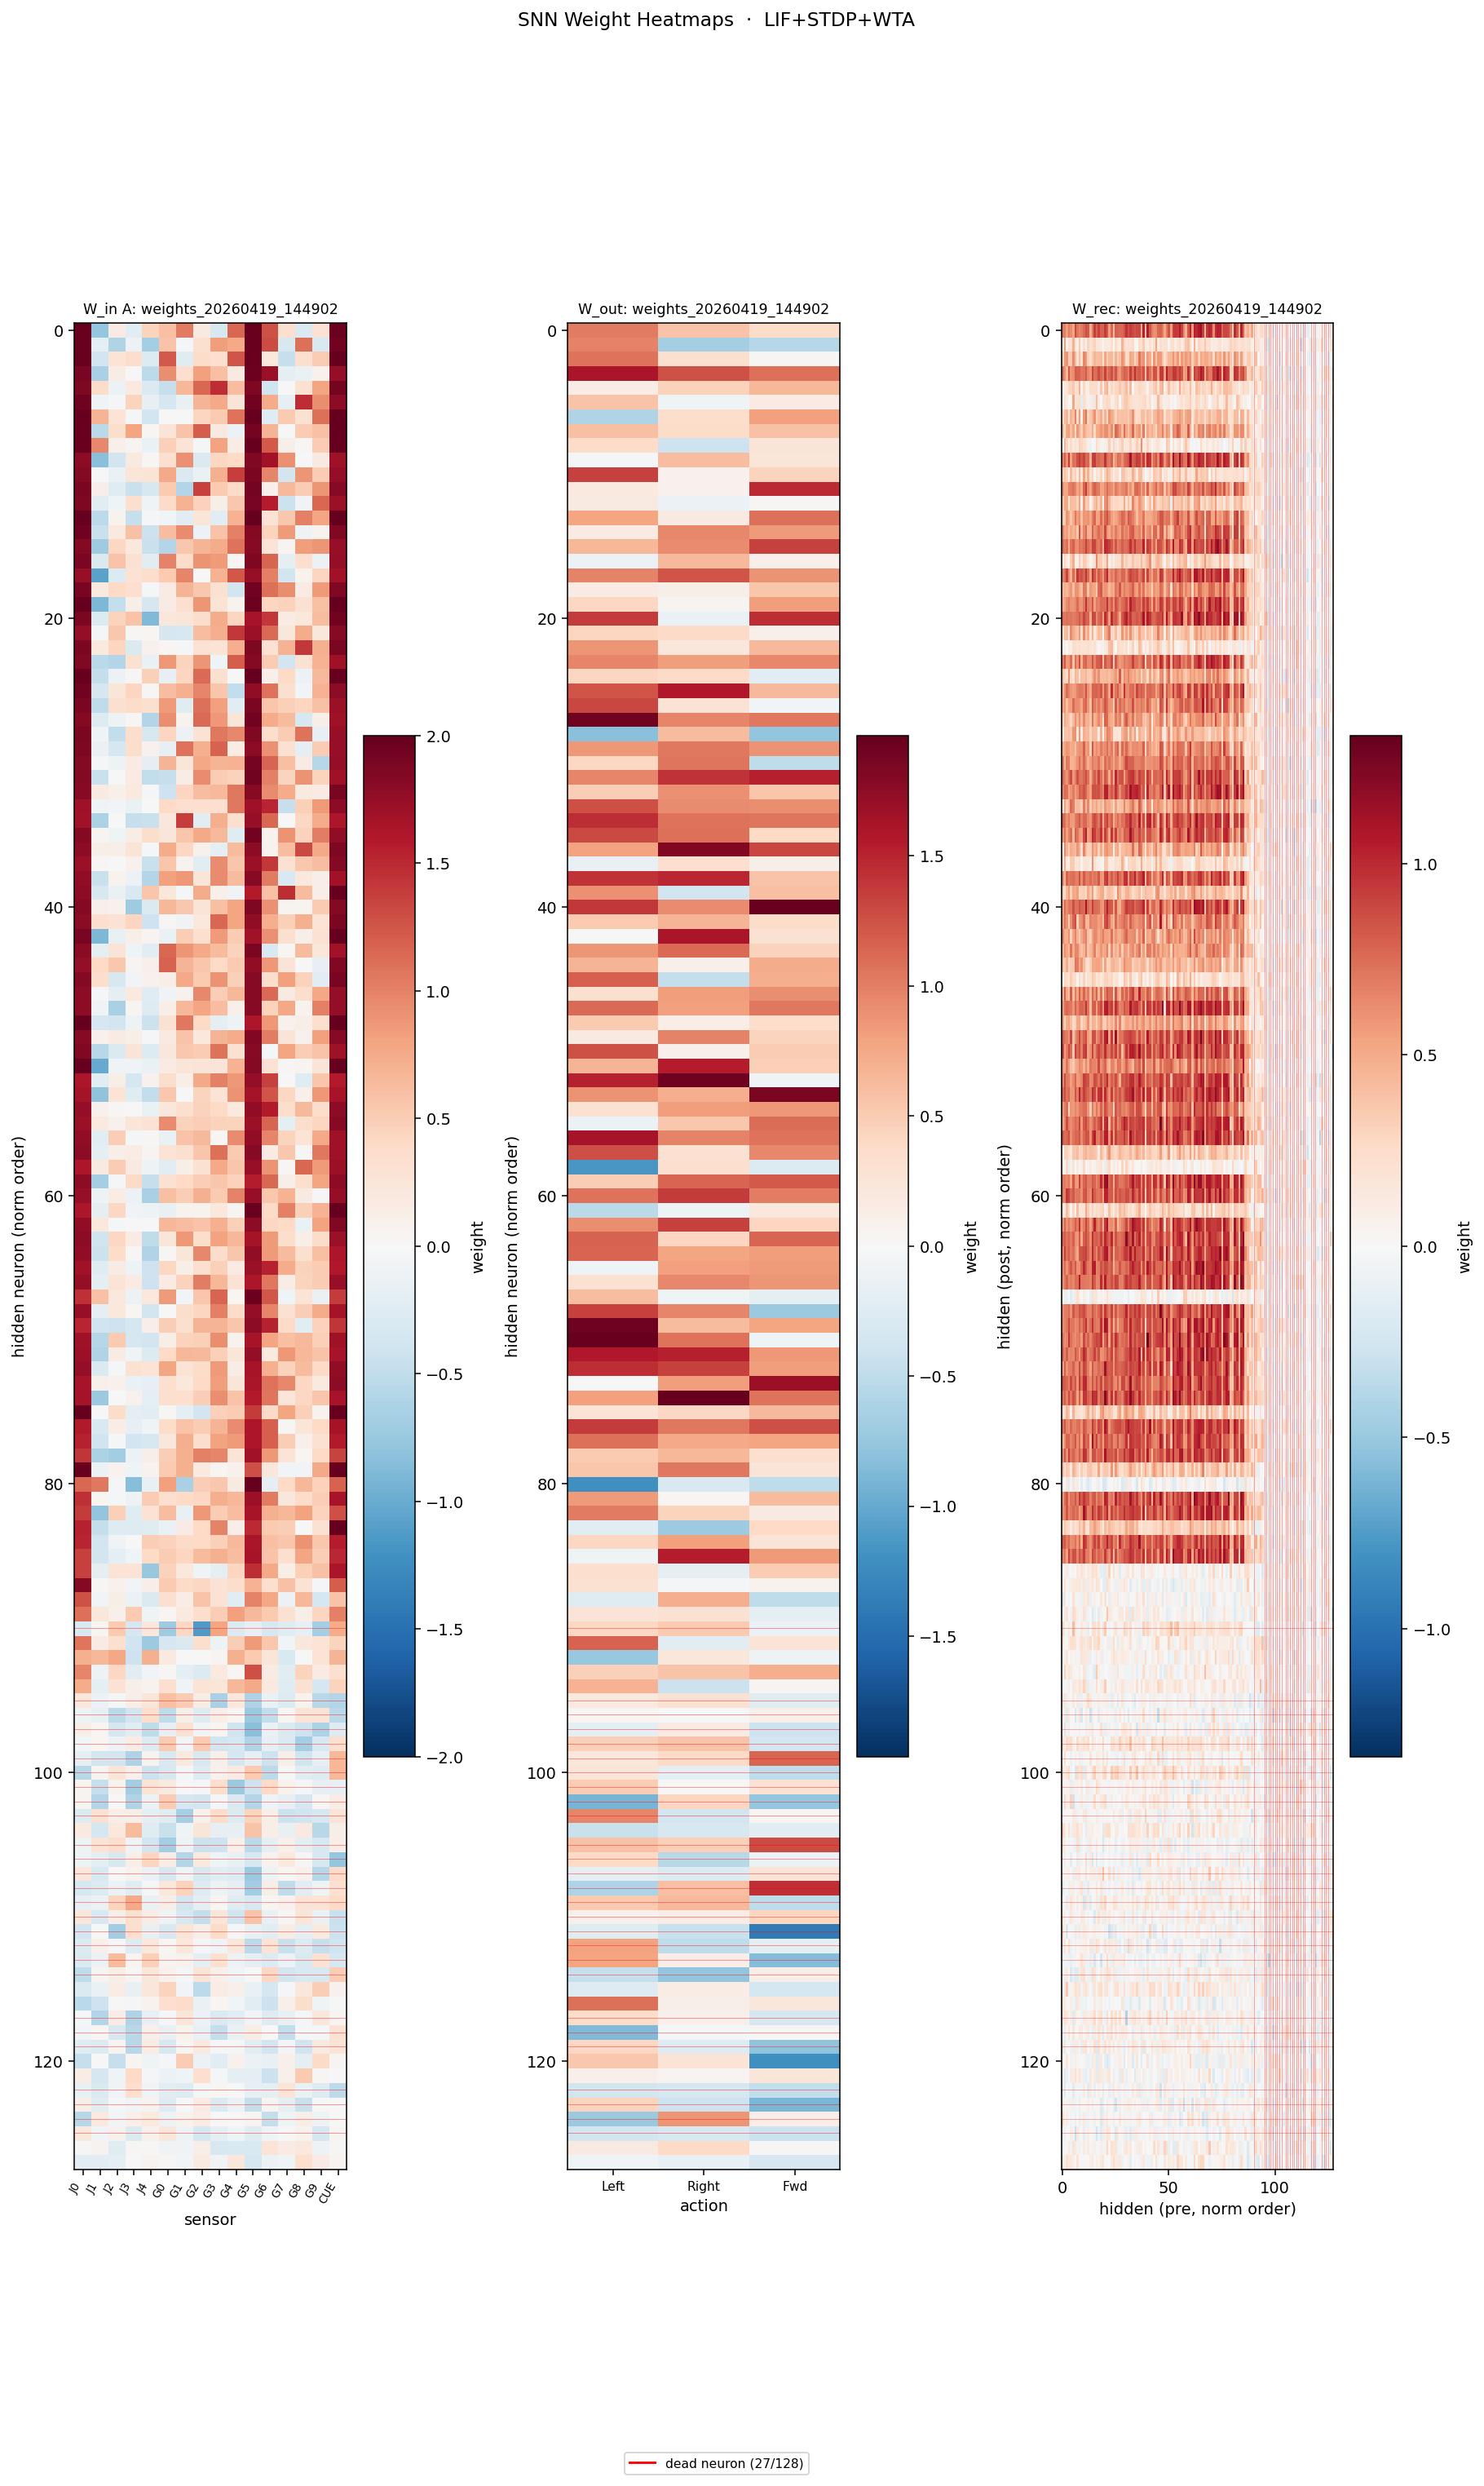
\includegraphics[width=0.7\linewidth]{fig1}
    \caption{Visualization of weights during Phase 1/2, showing extreme specialization to a single goal.}
    \label{fig:fig1}
\end{figure}

\subsection{Stage 2: Structural Recovery (Phase 3 with TRR)}
The control group (No-TRR) suffered catastrophic forgetting and resource depletion upon task switching (Figure 2). In contrast, the TRR group successfully reactivated almost all silent neurons, as shown in the top panel of Figure 6, achieving robust structural recovery.

\begin{figure}[htbp]
    \centering
    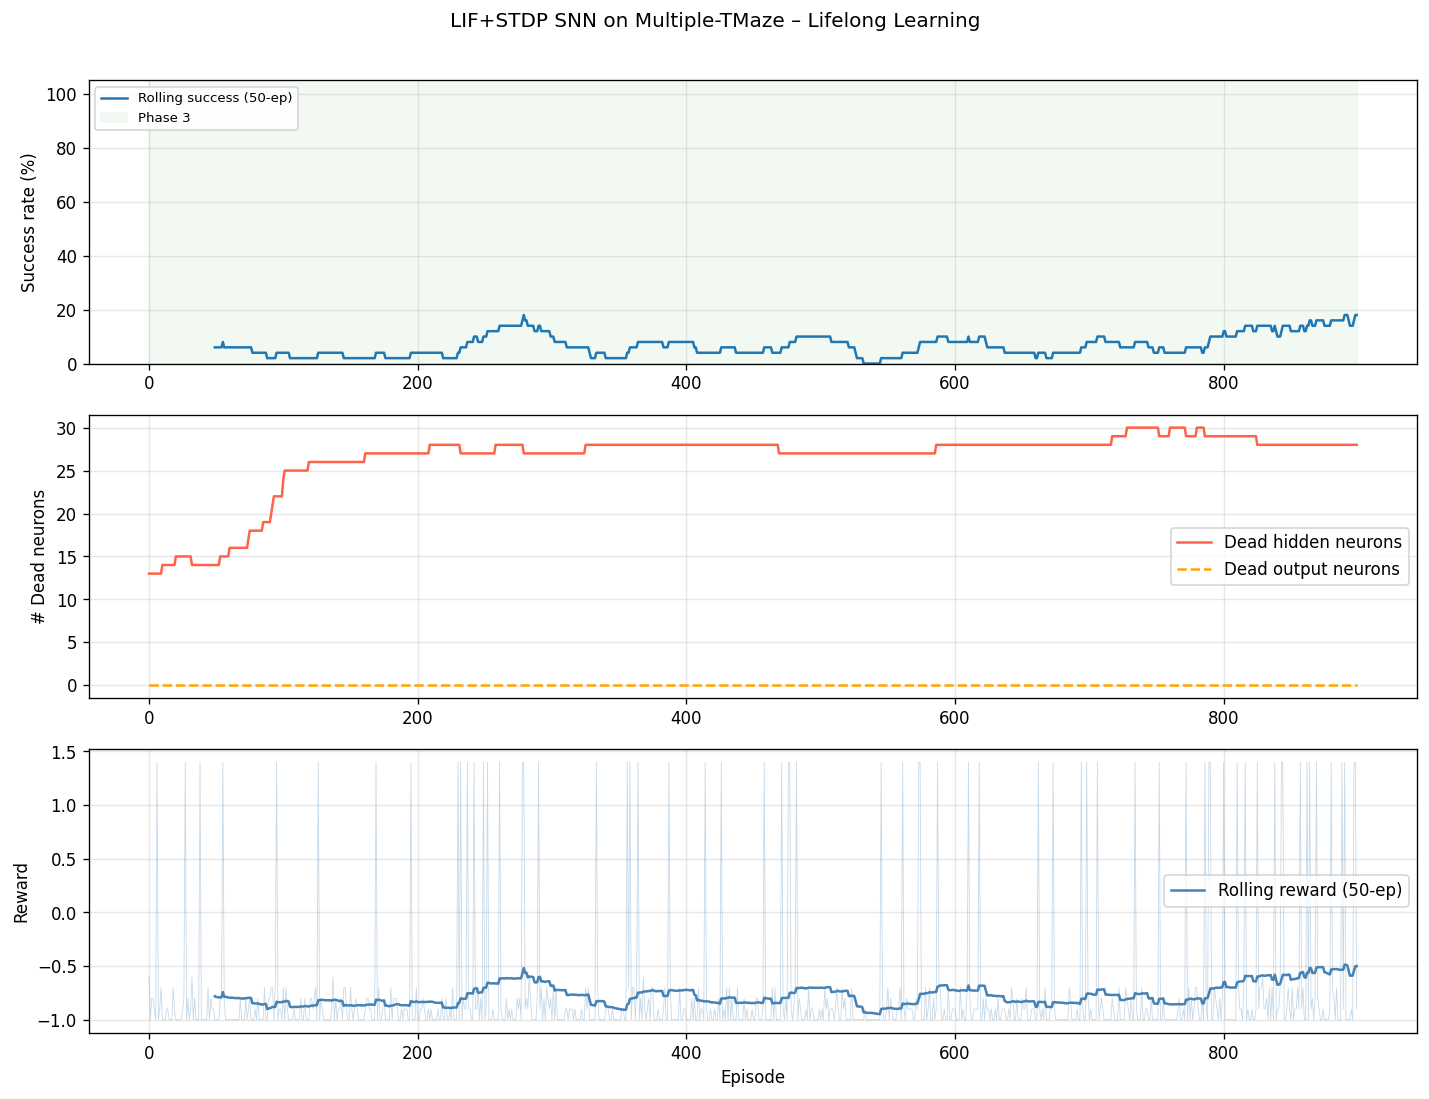
\includegraphics[width=0.45\linewidth]{fig2}
    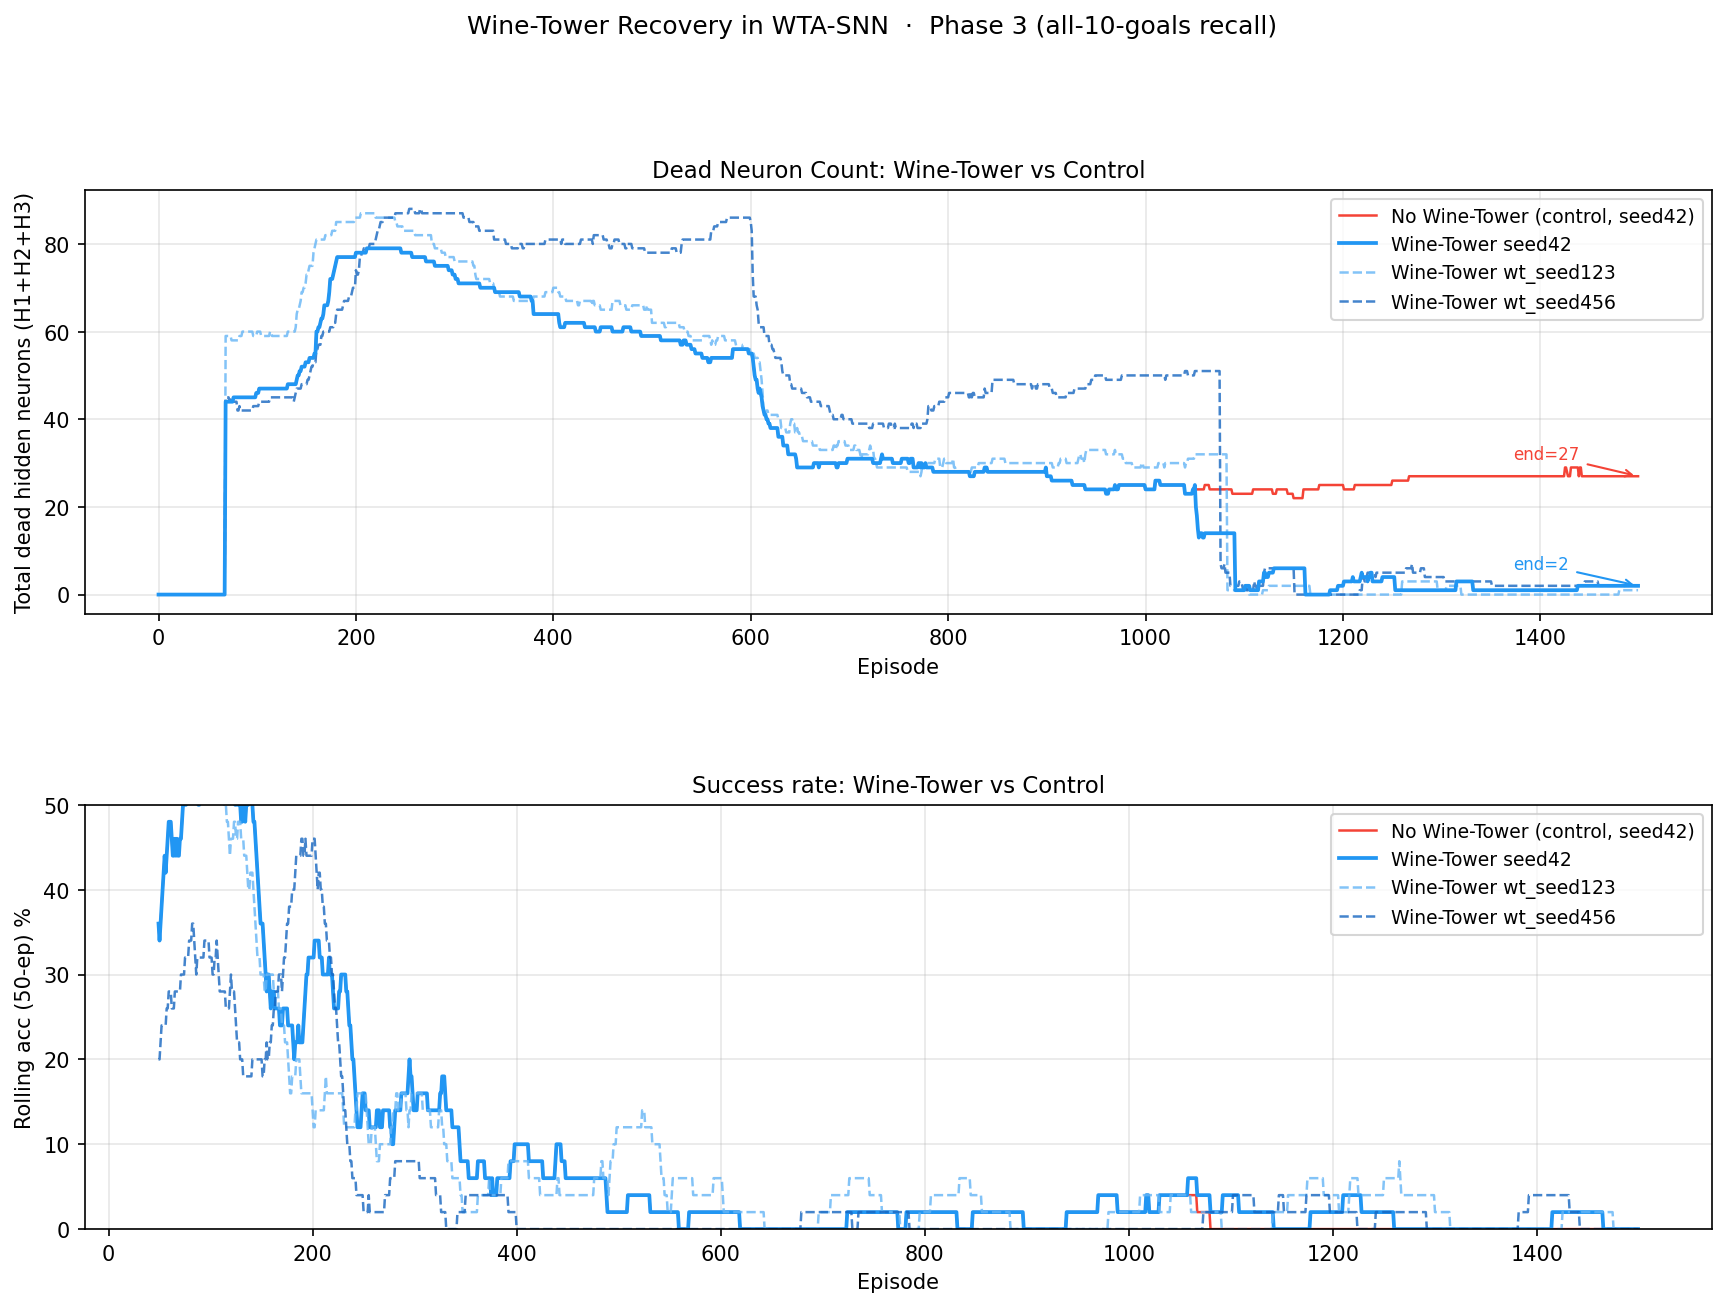
\includegraphics[width=0.45\linewidth]{fig6}
    \caption{Left: Resource depletion in No-TRR. Right: Dramatic structural recovery (top) and success rate transition (bottom) with TRR.}
    \label{fig:comparison_structural}
\end{figure}

\subsection{Stage 3: Functional Reintegration under Attractor Constraints}
However, the success rates in Figure 6 (bottom) revealed a crucial dissociation: structural recovery does not guarantee immediate functional plasticity. While neurons were revived, their activity was heavily constrained by the established WTA attractor basins, making it difficult to form independent representations for the novel task.

\section{Discussion: Dissociation of Structure and Function and Future Work}
The dissociation between structural recovery and functional adaptation highlights how attractor landscapes constrain plasticity in recurrent networks. Attractor basins carved deep by initial tasks forcibly absorb subsequent neural activity. To overcome this barrier, future work should incorporate metaplasticity mechanisms, such as temporarily scaling down pre-existing weights or adjusting firing thresholds, to destabilize consolidated attractors and allow new pathways to form.

\section{Conclusion}
The TRR model offers a robust structural solution to the dead-neuron problem in recurrent SNNs by utilizing local potential diffusion. While functional reintegration remains challenging due to attractor constraints, this study demonstrates that effective lifelong learning in recurrent SNNs requires both resource recovery and the dynamic modulation of attractor stability.

\bibliographystyle{plain}
\bibliography{references}
\end{document}
